%!TeX spellcheck = en-US
\documentclass[a4paper]{article}

\usepackage{fullpage} % Package to use full page
\usepackage{parskip} % Package to tweak paragraph skipping
\usepackage{tikz} % Package for drawing
\usepackage{amsmath}
\usepackage{amsfonts}
\usepackage{hyperref}
%\usepackage{threeparttable}
\usepackage{booktabs} % For tables
\usepackage{graphicx}
\usepackage{subcaption}
\usepackage{placeins}

\title{SF$3580$\\HW 2}
\author{Anna Broms \& Fredrik Fryklund}
\date{2018/11/29}

\begin{document}

\maketitle

<<<<<<< HEAD
 \section{Task $2$}
 %%!TeX spellcheck = en-US
%!TEX root = ../hw1_report.tex
As can be seen from Figure \ref{fig:task2} the rate of convergence is linear for the power method, as expected. For the Rayleigh quotient iteration the rate of convergence is cubic when $A$ is symmetric and quadratic when $A$ is nonsymmetric. This is also expected. The rate of convergence $p$ for the respective settings is approximated to $p\approx 3.03$ and $p \approx 2.2$, where
\begin{equation}
  p = \frac{\log{|\lambda^{(k+1)}-\lambda|}}{|\lambda^{(k)}-\lambda|}
\end{equation}
\begin{figure}[h!]
\centering
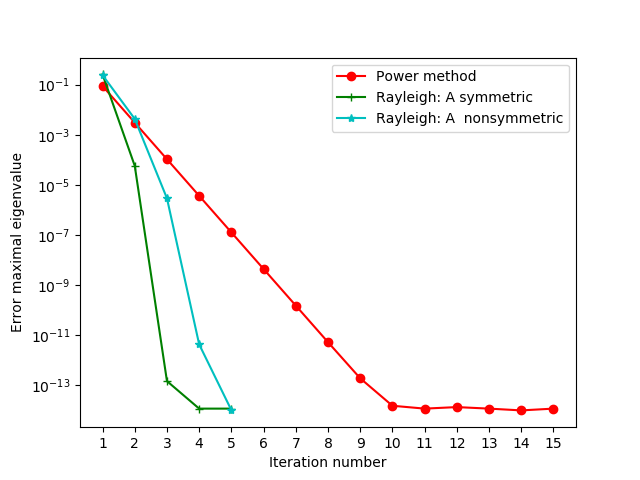
\includegraphics[scale=0.8]{../task2/task2.png}
\caption{Comparison of eigenvalues after $m$ iterations.}
\label{fig:task2}
\end{figure}

The Rayleigh quotient only uses the symmetric part of $A$ in
\begin{equation*}
  r(\mathbf{x}) = \mathbf{x}^{H}A\mathbf{x}
\end{equation*}
assuming $\mathbf{x}$ is normalized.
For $a_{13} = 4$ the matrix $A$ is no longer symmetric, i.e. $A\neq A^{H}$, but any square matrix can be decomposed into a symmetric part $A_{s}$ and a nonsymmetric part $A_{ns}$ by
\begin{equation}
  A = \underbrace{\frac{1}{2}\left(A + A^{H}\right)}_{= A_{s}} + \underbrace{\frac{1}{2}\left(A - A^{H}\right)}_{=A_{ns}}.
\end{equation}
Thus
\begin{equation*}
  r(\mathbf{x}) = \mathbf{x}^{H}A_{s}\mathbf{x} + \mathbf{x}^{H}A_{ns}\mathbf{x} = \mathbf{x}^{H}A_{s}\mathbf{x}
\end{equation*}
since
\begin{equation*}
 \mathbf{x}^{H}A_{ns}\mathbf{x}=\mathbf{x}^{H}A\mathbf{x} - \mathbf{x}^{H}A^{H}\mathbf{x} = 0.
\end{equation*}
For a nonsymmetric matrix all available information is not used.

%
 \section{Task $4$}
 %%!TeX spellcheck = en-US
%!TEX root = ../hw1_report.tex

We investigate a primitiv version of the Arnoldi method. Let 

 \section{Task $5$}
% %!TeX spellcheck = en-US
%!TEX root = ../hw2_report.tex


Given a real symmetric matrix $A$ with eigenvalues $10$, $10.5$ and 100 eigenvalues in the interval $[2,3]$, we prove a bound for then number of steps needed for CG to reduce the error measured in $\|Ax_n-b\|_{A^{-1}} = \|x_n-x_*\|$ by a factor $10^7$. We assume exact arithmetic and no breakdown.\\

\emph{Proof}:\\
Let $\kappa = \lambda_{\max}/ \lambda_{\min}$. By Theorem $38.5.$ in T.B. we have
\begin{equation}
  \label{task5:est1}
\frac{\|e_{n}\|}{\|e_{0}\|} = 2\left(\frac{\sqrt{\kappa}-1}{\sqrt{\kappa}+1}\right)^{n}.
\end{equation}
We seek $n$ such that the error has been reduced by a factor  $10^{7}$, i.e. $n$ such that \eqref{task5:est1} is about $1e-7$. For the matrix $A$ the largest lower bound for $\lambda_{\min}$ is $2$. The largest eigenvalue $\lambda_{\max} = 10.5$. We now solve the following problem for $n$,

\begin{align*}
&2\left(\frac{\sqrt{\kappa}-1}{\sqrt{\kappa}+1}\right)^{n}\leq 10^{-7}\\
&\\
\Leftrightarrow & n\leq\frac{\log{\left( 0.5\,10^{-7}}\right)}{\log{\left(\frac{\sqrt{\kappa}-1}{\sqrt{\kappa}+1}\right)}}
&\\
\Leftrightarrow & n\geq 17.967661670561174\\
&\\
\Leftrightarrow & n\geq 18.
\end{align*}
We confirm this numerically, $n = 17$ gives

\begin{equation*}
  2\left(\frac{\sqrt{\kappa}-1}{\sqrt{\kappa}+1}\right)^{18} \approx 2.473e-7
\end{equation*}

and $n = 18$ gives
\begin{equation*}
  2\left(\frac{\sqrt{\kappa}-1}{\sqrt{\kappa}+1}\right)^{18} \approx 9.702e-8.
\end{equation*}

 \section{Task $6$}
 %!TeX spellcheck = en-US
%!TEX root = ../hw1_report.tex
\subsection{(a)}
We compare GMRES and CGN for a given matrix $B$ and right hand side $b$. The result of the comparison is visualised in Figure \ref{task6}.

\subsection{(b)}
The result can be related to the convergence theory for CGN and GMRES.

\section{Task $7$}
%%!TeX spellcheck = en-US
%!TEX root = ../hw3_report.tex
\subsection*{(a)}
%We start by observing that if $\lambda$ and $v$ are an eigenpair for $A$, then $t\lambda$ is an eigenvalue of $tA$ since $tAv = t\lambda v$.
%
%Let $\mu \in \mathbb{C}$ be an expansion point, then
%\begin{equation}
%  f(tA) = \sum\limits_{i = 0}^{\infty} \frac{f^{(i)}(\mu)}{i!}(tA-\mu I)^{i}.
%\end{equation}
%If $A\in\mathbb{C}^{n\times n}$, then $f:C^{n \times n}\rightarrow C^{n \times n}$. Let $f(z) = \exp (z)$ and $g(z) = dz(t)/dt$, then
%\begin{equation}
%  g(f(tA)) = g\left(\sum\limits_{i = 0}^{\infty} \frac{\exp(\mu)}{i!}(tA-\mu I)^{i}\right) = \sum\limits_{i = 0}^{\infty}\left( \frac{\exp(\mu)}{i!}g((tA-\mu I)^{i})\right) = A\sum\limits_{i = 1}^{\infty}\frac{\exp(\mu)}{(i-1)!}\left(tA-\mu I\right)^{i-1},
%\end{equation}
%be rearranging the indices since $(tA-\mu I)^{0} = I$. The above holds if $g((tA)^{i}) = iA(tA)^{i-1}$. How to show this?

%Anna's attempt:
Consider the function $f(z,t) = e^{tz}$. We want to investigate the matrix valued function $f(A,t) = e^{Az}$. Let $\mu \in \mathbb{C}$ be an expansion point. Then,
\begin{equation}
  f(A,t) = \sum\limits_{i = 0}^{\infty} \frac{f^{(i)}(\mu)}{i!}(A-\mu I)^{i} = \sum\limits_{i = 0}^{\infty} \frac{t^ie^{t\mu}}{i!}(A-\mu I)^{i}.
\end{equation}
If $A\in\mathbb{C}^{n\times n}$, then $f:C^{n \times n}\rightarrow C^{n \times n}$. Now, compute the derivative of $f(A,t)$ with respect to time:
\begin{equation}
\begin{aligned}
\frac{\mathrm d}{\mathrm d t}e^{tA} & = \frac{\mathrm d}{\mathrm dt}\sum^{\infty}_{i = 0} \frac{t^ie^{t\mu}}{i!}(A-\mu I )^i = \\
& = \sum^{\infty}_{i = 0} \frac{\mathrm d}{\mathrm dt}\left(\frac{t^ie^{t\mu}}{i!}(A-\mu I )^i\right) = \\
& = \sum^{\infty}_{i = 0} \frac{\mathrm d}{\mathrm dt}\left(\frac{t^ie^{t\mu}}{i!}\right)(A-\mu I )^i  = \\
&= \sum^{\infty}_{i = 0}  \left(\frac{it^{i-1}e^{t\mu}+t^i\mu e^{t\mu}}{i!}\right) (A-\mu I )^i.
\end{aligned}
\end{equation}
The last expression can be identified as $g(A)$, where $g(z) = ze^{tz}$ as  the expression
\begin{equation}
\left(it^{i-1}e^{t\mu}+t^i\mu e^{t\mu}\right)
\end{equation}
is the $i$th derivative of the product $z\cdot e^{tz}$, which can be seen using the general Leibniz rule ($(f_1f_2)^{(n)} = \sum_{k = 0}^n\binom{n}{k}f_1^{(n-k)}(x)f_2^{(k)}(x)$). Thus, we can conclude that $\frac{\mathrm d }{\mathrm dt}e^{tA} = Ae^{tA}$. The matrix function $e^{tA}A$ has the same Taylor expansion expression as $Ae^{tA}$. Thus, $\frac{\mathrm d }{\mathrm dt}e^{tA} = Ae^{tA} = e^{tA} A$, which is what we wanted to show.




%Let $f(z) = \exp (z)$ and $g(z) = dz(t)/dt$, then
%\begin{equation}
%  g(f(tA)) = g\left(\sum\limits_{i = 0}^{\infty} \frac{\exp(\mu)}{i!}(tA-\mu I)^{i}\right) = \sum\limits_{i = 0}^{\infty}\left( \frac{\exp(\mu)}{i!}g((tA-\mu I)^{i})\right) = A\sum\limits_{i = 1}^{\infty}\frac{\exp(\mu)}{(i-1)!}\left(tA-\mu I\right)^{i-1},
%\end{equation}
%be rearranging the indices since $(tA-\mu I)^{0} = I$. The above holds if $g((tA)^{i}) = iA(tA)^{i-1}$. How to show this?
\subsection*{(b)}
Introduce
\begin{equation}
[B,A]_{n} =  [[B,A]_{n-1},A], n = 0,1,2,\ldots, \quad \text{ where }[B,A]_{1} = [B,A] = BA-AB \text{ and } [B,A]_{0} = B,
\end{equation}
which satisfies $[A+B,C]_{n} = [A,C]_{n} + [B,C]_{n}$. This is shown by induction: the initial case is $[A+B,C]_{1} = AC-CA + BC-CB = [A,C]_{1}+[B,C]_{1}$. Now assume $[A+B,C]_{n} = [A,C]_{n} + [B,C]_{n}$ holds, then
\begin{align}
[A+B,C]_{n+1} &=  [AC-CA + BC-CB,A]_{n} = [AC-CA,C]_{n} + [BC-CB,C]_{n} \\
&= [[A,C],C]_{n} + [[B,C],C]_{n}=[A,C]_{n+1} + [B,C]_{n+1}.
\end{align}


Let $G(t) = \exp(-tA)B\exp(tA)$, which is analytic in $t$. Thus we may write
\begin{equation}
  \label{eq:task7bTaylor}
G(t) = \sum\limits_{i = 0}^{\infty}\frac{t^{i}}{i!} G^{(i)}(\mu)=\sum\limits_{i = 0}^{\infty}\frac{t^{i}}{i!} G_{i},
\end{equation}
where $G_{0} = B$.
By (a) we have that
\begin{equation}
  \frac{d}{dt}G(t) = G(t)A-AG(T) = [G(t),A].
\end{equation}
Setting this to be equal to the the derivative of \eqref{eq:task7bTaylor} with respect to $t$ gives
\begin{equation}
\sum\limits_{i = 0}^{\infty}\frac{t^{i}}{i!} [G_{i},A] = \sum\limits_{i = 1}^{\infty}\frac{t^{i-1}}{(i-1)!} G_{i}.
\end{equation}
By shifting the indexing from $i = 1,2,\ldots $ to $i = 0,1,\ldots$ for the right hand side we get
\begin{equation}
\sum\limits_{i = 0}^{\infty}\frac{t^{i}}{i!} [G_{i},A] = \sum\limits_{i = 0}^{\infty}\frac{t^{i}}{i!} G_{i+1}.
\end{equation}
We conclude that $G_{i+1} = [G_{i},A]_{i}$, that is $G_{1} = [G_{0},A]_{0} = B$ and
\begin{equation}
  G(t) = B + t[B,A]+\frac{t^{2}}{2!}[[B,A],A]+\frac{t^{2}}{2!}[[B,A],A,A]+\ldots
\end{equation}


\subsection*{(d)}
Task: Let $C_k = [C_{k-1},A]$, with $C_0 = B$. We want to show that $\|C_k\|\leq 2^k\|A\|^k\|B\|$.

The proof is done by induction. For $k = 0$ we have that $\|C_0\| = \|B\|\leq 2^0\|A\|^0\|B\|$. Now, assume that $\|C_k\|\leq 2^k\|A\|^k\|B\|$. We want to show that
$\|C_{k+1}\|\leq 2^{k+1}\|A\|^{k+1}\|B\|$:

\begin{equation}
\begin{aligned}
\|C_{k+1}\| = \|C_kA-AC_k\| = \|C_{k}A+(-AC_k)\|\leq\|C_kA\|+\|-AC_k\| = \|C_kA+|-1|\|AC_k\|\leq\|C_k\|\|A\|+\|A\|\|C_k\| =\\
= 2\|A\|\|C_k\| = 2^{k+1}\|A\|^{k+1}\|B\|,
\end{aligned}
\end{equation}
which is what we wanted to show.
\subsection*{(e)}
Suppose $\|A\|<\frac{1}{2}$ and $t\leq 1$. Let $G_N(t)$ be the truncation of $G(t)$, where
\begin{equation}
G(t) = \sum^{\infty}_{k = 0}\frac{t^k}{k!}C_k.
\end{equation}
Then,
\begin{equation}
\begin{aligned}
\|G_N(t)-G(t)\|&= \|\sum^{\infty}_{k = N+1}\frac{t^k}{k!}C_k\|\leq\sum^{\infty}_{k = N+1}\left(\frac{t^k}{k!}\right)\|C_k\|\leq\\
&\leq \sum^{\infty}_{k = N+1}\left(\frac{t^k}{k!}\right)2^k\|A\|^k\|B\|\leq \sum^{\infty}_{k = N+1}\left(\frac{t^k}{k!}\right)2^k\left(\frac{1}{2}\right)^2\|B\|\leq\frac{\|B\|}{(N+1)!}\sum^{\infty}_{k = N+1}t^k = \frac{\|B\|}{(N+1)!}\sum^{\infty}_{k = 0}t^{k+(N+1)} =\\&=\frac{\|B\|t^{N-1}}{(N+1)!}t^{N+1}\cdot\frac{1}{1-t}.
\end{aligned}
\end{equation}

=======
 \section*{Task $2$}
 %!TeX spellcheck = en-US
%!TEX root = ../hw1_report.tex
As can be seen from Figure \ref{fig:task2} the rate of convergence is linear for the power method, as expected. For the Rayleigh quotient iteration the rate of convergence is cubic when $A$ is symmetric and quadratic when $A$ is nonsymmetric. This is also expected. The rate of convergence $p$ for the respective settings is approximated to $p\approx 3.03$ and $p \approx 2.2$, where
\begin{equation}
  p = \frac{\log{|\lambda^{(k+1)}-\lambda|}}{|\lambda^{(k)}-\lambda|}
\end{equation}
\begin{figure}[h!]
\centering
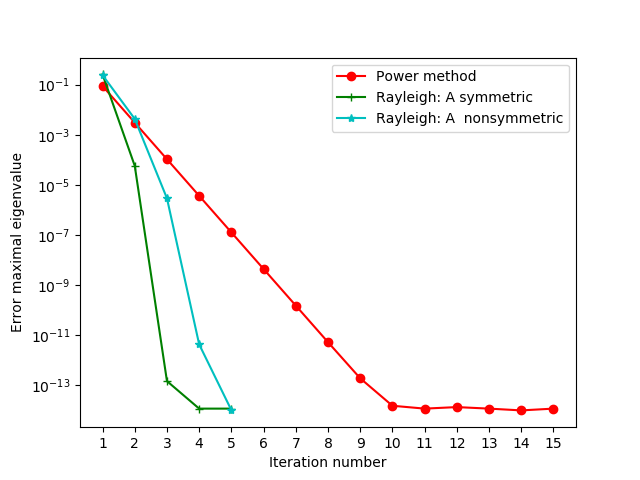
\includegraphics[scale=0.8]{../task2/task2.png}
\caption{Comparison of eigenvalues after $m$ iterations.}
\label{fig:task2}
\end{figure}

The Rayleigh quotient only uses the symmetric part of $A$ in
\begin{equation*}
  r(\mathbf{x}) = \mathbf{x}^{H}A\mathbf{x}
\end{equation*}
assuming $\mathbf{x}$ is normalized.
For $a_{13} = 4$ the matrix $A$ is no longer symmetric, i.e. $A\neq A^{H}$, but any square matrix can be decomposed into a symmetric part $A_{s}$ and a nonsymmetric part $A_{ns}$ by
\begin{equation}
  A = \underbrace{\frac{1}{2}\left(A + A^{H}\right)}_{= A_{s}} + \underbrace{\frac{1}{2}\left(A - A^{H}\right)}_{=A_{ns}}.
\end{equation}
Thus
\begin{equation*}
  r(\mathbf{x}) = \mathbf{x}^{H}A_{s}\mathbf{x} + \mathbf{x}^{H}A_{ns}\mathbf{x} = \mathbf{x}^{H}A_{s}\mathbf{x}
\end{equation*}
since
\begin{equation*}
 \mathbf{x}^{H}A_{ns}\mathbf{x}=\mathbf{x}^{H}A\mathbf{x} - \mathbf{x}^{H}A^{H}\mathbf{x} = 0.
\end{equation*}
For a nonsymmetric matrix all available information is not used.

%
 \section*{Task $4$}
 %!TeX spellcheck = en-US
%!TEX root = ../hw1_report.tex

We investigate a primitiv version of the Arnoldi method. Let 

 \section*{Task $5$}
 %!TeX spellcheck = en-US
%!TEX root = ../hw2_report.tex


Given a real symmetric matrix $A$ with eigenvalues $10$, $10.5$ and 100 eigenvalues in the interval $[2,3]$, we prove a bound for then number of steps needed for CG to reduce the error measured in $\|Ax_n-b\|_{A^{-1}} = \|x_n-x_*\|$ by a factor $10^7$. We assume exact arithmetic and no breakdown.\\

\emph{Proof}:\\
Let $\kappa = \lambda_{\max}/ \lambda_{\min}$. By Theorem $38.5.$ in T.B. we have
\begin{equation}
  \label{task5:est1}
\frac{\|e_{n}\|}{\|e_{0}\|} = 2\left(\frac{\sqrt{\kappa}-1}{\sqrt{\kappa}+1}\right)^{n}.
\end{equation}
We seek $n$ such that the error has been reduced by a factor  $10^{7}$, i.e. $n$ such that \eqref{task5:est1} is about $1e-7$. For the matrix $A$ the largest lower bound for $\lambda_{\min}$ is $2$. The largest eigenvalue $\lambda_{\max} = 10.5$. We now solve the following problem for $n$,

\begin{align*}
&2\left(\frac{\sqrt{\kappa}-1}{\sqrt{\kappa}+1}\right)^{n}\leq 10^{-7}\\
&\\
\Leftrightarrow & n\leq\frac{\log{\left( 0.5\,10^{-7}}\right)}{\log{\left(\frac{\sqrt{\kappa}-1}{\sqrt{\kappa}+1}\right)}}
&\\
\Leftrightarrow & n\geq 17.967661670561174\\
&\\
\Leftrightarrow & n\geq 18.
\end{align*}
We confirm this numerically, $n = 17$ gives

\begin{equation*}
  2\left(\frac{\sqrt{\kappa}-1}{\sqrt{\kappa}+1}\right)^{18} \approx 2.473e-7
\end{equation*}

and $n = 18$ gives
\begin{equation*}
  2\left(\frac{\sqrt{\kappa}-1}{\sqrt{\kappa}+1}\right)^{18} \approx 9.702e-8.
\end{equation*}

 \section*{Task $6$}
 %!TeX spellcheck = en-US
%!TEX root = ../hw1_report.tex
\subsection{(a)}
We compare GMRES and CGN for a given matrix $B$ and right hand side $b$. The result of the comparison is visualised in Figure \ref{task6}.

\subsection{(b)}
The result can be related to the convergence theory for CGN and GMRES.

\section*{Task $7$}
%!TeX spellcheck = en-US
%!TEX root = ../hw3_report.tex
\subsection*{(a)}
%We start by observing that if $\lambda$ and $v$ are an eigenpair for $A$, then $t\lambda$ is an eigenvalue of $tA$ since $tAv = t\lambda v$.
%
%Let $\mu \in \mathbb{C}$ be an expansion point, then
%\begin{equation}
%  f(tA) = \sum\limits_{i = 0}^{\infty} \frac{f^{(i)}(\mu)}{i!}(tA-\mu I)^{i}.
%\end{equation}
%If $A\in\mathbb{C}^{n\times n}$, then $f:C^{n \times n}\rightarrow C^{n \times n}$. Let $f(z) = \exp (z)$ and $g(z) = dz(t)/dt$, then
%\begin{equation}
%  g(f(tA)) = g\left(\sum\limits_{i = 0}^{\infty} \frac{\exp(\mu)}{i!}(tA-\mu I)^{i}\right) = \sum\limits_{i = 0}^{\infty}\left( \frac{\exp(\mu)}{i!}g((tA-\mu I)^{i})\right) = A\sum\limits_{i = 1}^{\infty}\frac{\exp(\mu)}{(i-1)!}\left(tA-\mu I\right)^{i-1},
%\end{equation}
%be rearranging the indices since $(tA-\mu I)^{0} = I$. The above holds if $g((tA)^{i}) = iA(tA)^{i-1}$. How to show this?

%Anna's attempt:
Consider the function $f(z,t) = e^{tz}$. We want to investigate the matrix valued function $f(A,t) = e^{Az}$. Let $\mu \in \mathbb{C}$ be an expansion point. Then,
\begin{equation}
  f(A,t) = \sum\limits_{i = 0}^{\infty} \frac{f^{(i)}(\mu)}{i!}(A-\mu I)^{i} = \sum\limits_{i = 0}^{\infty} \frac{t^ie^{t\mu}}{i!}(A-\mu I)^{i}.
\end{equation}
If $A\in\mathbb{C}^{n\times n}$, then $f:C^{n \times n}\rightarrow C^{n \times n}$. Now, compute the derivative of $f(A,t)$ with respect to time:
\begin{equation}
\begin{aligned}
\frac{\mathrm d}{\mathrm d t}e^{tA} & = \frac{\mathrm d}{\mathrm dt}\sum^{\infty}_{i = 0} \frac{t^ie^{t\mu}}{i!}(A-\mu I )^i = \\
& = \sum^{\infty}_{i = 0} \frac{\mathrm d}{\mathrm dt}\left(\frac{t^ie^{t\mu}}{i!}(A-\mu I )^i\right) = \\
& = \sum^{\infty}_{i = 0} \frac{\mathrm d}{\mathrm dt}\left(\frac{t^ie^{t\mu}}{i!}\right)(A-\mu I )^i  = \\
&= \sum^{\infty}_{i = 0}  \left(\frac{it^{i-1}e^{t\mu}+t^i\mu e^{t\mu}}{i!}\right) (A-\mu I )^i.
\end{aligned}
\end{equation}
The last expression can be identified as $g(A)$, where $g(z) = ze^{tz}$ as  the expression
\begin{equation}
\left(it^{i-1}e^{t\mu}+t^i\mu e^{t\mu}\right)
\end{equation}
is the $i$th derivative of the product $z\cdot e^{tz}$, which can be seen using the general Leibniz rule ($(f_1f_2)^{(n)} = \sum_{k = 0}^n\binom{n}{k}f_1^{(n-k)}(x)f_2^{(k)}(x)$). Thus, we can conclude that $\frac{\mathrm d }{\mathrm dt}e^{tA} = Ae^{tA}$. The matrix function $e^{tA}A$ has the same Taylor expansion expression as $Ae^{tA}$. Thus, $\frac{\mathrm d }{\mathrm dt}e^{tA} = Ae^{tA} = e^{tA} A$, which is what we wanted to show.




%Let $f(z) = \exp (z)$ and $g(z) = dz(t)/dt$, then
%\begin{equation}
%  g(f(tA)) = g\left(\sum\limits_{i = 0}^{\infty} \frac{\exp(\mu)}{i!}(tA-\mu I)^{i}\right) = \sum\limits_{i = 0}^{\infty}\left( \frac{\exp(\mu)}{i!}g((tA-\mu I)^{i})\right) = A\sum\limits_{i = 1}^{\infty}\frac{\exp(\mu)}{(i-1)!}\left(tA-\mu I\right)^{i-1},
%\end{equation}
%be rearranging the indices since $(tA-\mu I)^{0} = I$. The above holds if $g((tA)^{i}) = iA(tA)^{i-1}$. How to show this?
\subsection*{(b)}
Introduce
\begin{equation}
[B,A]_{n} =  [[B,A]_{n-1},A], n = 0,1,2,\ldots, \quad \text{ where }[B,A]_{1} = [B,A] = BA-AB \text{ and } [B,A]_{0} = B,
\end{equation}
which satisfies $[A+B,C]_{n} = [A,C]_{n} + [B,C]_{n}$. This is shown by induction: the initial case is $[A+B,C]_{1} = AC-CA + BC-CB = [A,C]_{1}+[B,C]_{1}$. Now assume $[A+B,C]_{n} = [A,C]_{n} + [B,C]_{n}$ holds, then
\begin{align}
[A+B,C]_{n+1} &=  [AC-CA + BC-CB,A]_{n} = [AC-CA,C]_{n} + [BC-CB,C]_{n} \\
&= [[A,C],C]_{n} + [[B,C],C]_{n}=[A,C]_{n+1} + [B,C]_{n+1}.
\end{align}


Let $G(t) = \exp(-tA)B\exp(tA)$, which is analytic in $t$. Thus we may write
\begin{equation}
  \label{eq:task7bTaylor}
G(t) = \sum\limits_{i = 0}^{\infty}\frac{t^{i}}{i!} G^{(i)}(\mu)=\sum\limits_{i = 0}^{\infty}\frac{t^{i}}{i!} G_{i},
\end{equation}
where $G_{0} = B$.
By (a) we have that
\begin{equation}
  \frac{d}{dt}G(t) = G(t)A-AG(T) = [G(t),A].
\end{equation}
Setting this to be equal to the the derivative of \eqref{eq:task7bTaylor} with respect to $t$ gives
\begin{equation}
\sum\limits_{i = 0}^{\infty}\frac{t^{i}}{i!} [G_{i},A] = \sum\limits_{i = 1}^{\infty}\frac{t^{i-1}}{(i-1)!} G_{i}.
\end{equation}
By shifting the indexing from $i = 1,2,\ldots $ to $i = 0,1,\ldots$ for the right hand side we get
\begin{equation}
\sum\limits_{i = 0}^{\infty}\frac{t^{i}}{i!} [G_{i},A] = \sum\limits_{i = 0}^{\infty}\frac{t^{i}}{i!} G_{i+1}.
\end{equation}
We conclude that $G_{i+1} = [G_{i},A]_{i}$, that is $G_{1} = [G_{0},A]_{0} = B$ and
\begin{equation}
  G(t) = B + t[B,A]+\frac{t^{2}}{2!}[[B,A],A]+\frac{t^{2}}{2!}[[B,A],A,A]+\ldots
\end{equation}


\subsection*{(d)}
Task: Let $C_k = [C_{k-1},A]$, with $C_0 = B$. We want to show that $\|C_k\|\leq 2^k\|A\|^k\|B\|$.

The proof is done by induction. For $k = 0$ we have that $\|C_0\| = \|B\|\leq 2^0\|A\|^0\|B\|$. Now, assume that $\|C_k\|\leq 2^k\|A\|^k\|B\|$. We want to show that
$\|C_{k+1}\|\leq 2^{k+1}\|A\|^{k+1}\|B\|$:

\begin{equation}
\begin{aligned}
\|C_{k+1}\| = \|C_kA-AC_k\| = \|C_{k}A+(-AC_k)\|\leq\|C_kA\|+\|-AC_k\| = \|C_kA+|-1|\|AC_k\|\leq\|C_k\|\|A\|+\|A\|\|C_k\| =\\
= 2\|A\|\|C_k\| = 2^{k+1}\|A\|^{k+1}\|B\|,
\end{aligned}
\end{equation}
which is what we wanted to show.
\subsection*{(e)}
Suppose $\|A\|<\frac{1}{2}$ and $t\leq 1$. Let $G_N(t)$ be the truncation of $G(t)$, where
\begin{equation}
G(t) = \sum^{\infty}_{k = 0}\frac{t^k}{k!}C_k.
\end{equation}
Then,
\begin{equation}
\begin{aligned}
\|G_N(t)-G(t)\|&= \|\sum^{\infty}_{k = N+1}\frac{t^k}{k!}C_k\|\leq\sum^{\infty}_{k = N+1}\left(\frac{t^k}{k!}\right)\|C_k\|\leq\\
&\leq \sum^{\infty}_{k = N+1}\left(\frac{t^k}{k!}\right)2^k\|A\|^k\|B\|\leq \sum^{\infty}_{k = N+1}\left(\frac{t^k}{k!}\right)2^k\left(\frac{1}{2}\right)^2\|B\|\leq\frac{\|B\|}{(N+1)!}\sum^{\infty}_{k = N+1}t^k = \frac{\|B\|}{(N+1)!}\sum^{\infty}_{k = 0}t^{k+(N+1)} =\\&=\frac{\|B\|t^{N-1}}{(N+1)!}t^{N+1}\cdot\frac{1}{1-t}.
\end{aligned}
\end{equation}

>>>>>>> 0bf53df848f038c911080f8c1922430ca706ee59

\end{document}
